
\section{Model} 


I present a heterogenous agents model with human capital dynamics, search and matching frictions, and nominal rigidities. 

\subsection{Households}
\label{subsec:Households}

There is a continuum of households of mass 1 indexed by $i$ who face both idiosyncratic permanent and transitory income shocks, stochastic transitions between employment and unemployment, and is subject to human capital accumulation or erosion. A household's employment state is indexed by $n_{it}$. Employed households ($n_{it} = 1$) receive a wage $w_{t}$ that is taxed at rate $\tau_{t}$, accumulate human capital $h_{it}$ with probability $\pi_{L}$, and separate from employment with probability $\omega$. If an employed household is separated, he finds a job in the same period with probability $\eta_{r,t}$ or else he transitions to unemployment ($n_{it} = 0$).  When a household becomes unemployed, he randomly enters one of three unemployment states $X_{it}$. A household is either a permanent layoff (P), a temporary layoff (T), or a quitter/other (O). The probability of entering each state is $\lambda(X)$ where $X \in \{ P , T , O \}$. As in \cite{Gertler2022}, households who are in temporary layoff can transition to a permanent layoff with probability $p_{TLPL}$.  During a permanent or temporary layoff spell, households receive unemployment benefits that expire after $\bar{d}$ periods. Quitters/other types of unemployment do not receive unemployment benefits. During unemployment, a household in unemployed state $X_{it}$ finds employment with probability $\eta_{t}(X_{it})$. Only households who reenter employment from a permanent layoff have a probability of experiencing human capital erosion that is realized during the new employment spell. In addition, households are subject to a constant probability of death (perpetual youth) and are ex-ante heterogeneous in their discount factors. After all shocks and transitions are realized, households choose to consume and save into government bonds. \\ 

The timing of the household problem is illustrated in figure \ref{Model Timing}

    
\begin{figure}[!ht]
\begin{scriptsize}
\begin{center}
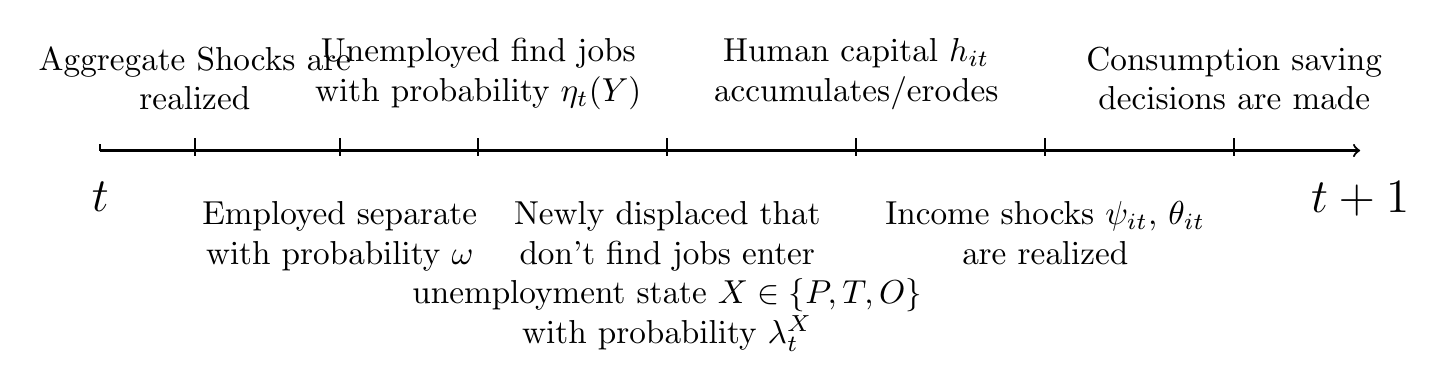
\begin{tikzpicture}[thick,scale=.8, every node/.style={scale=1.2}]
  \draw[->] (-5,0) -- (15,0)  ;
  \draw (15,-.3) node[below] {\Large $t+1$};
  \draw (-5,0) node{}  -- (-5,0.1);
  \draw (-5,-.3) node[below] {\Large $t$};
  \draw (-3.5,-.08) node[above=10pt,align=center] {Aggregate Shocks are\\realized} -- (-3.5,0.2);
    \draw (-1.2,-.08) node[below=10pt,align=center] {Employed separate\\ with probability $\omega$} -- (-1.2,.2);
  \draw (1.,-.08) node[above=10pt,align=center] {Unemployed find jobs\\with probability $\eta_{t}(Y)$ } -- (1,0.2);
   \draw (4.,-.08) node[below=10pt,align=center] {Newly displaced that \\ don't find jobs enter \\ unemployment state $X \in \{ P , T , O \} $\\ with probability $\lambda^{X}_{t}$} -- (4.,0.2);
  \draw (7.,-.08) node[above=10pt,align=center] {Human capital $h_{it}$ \\ accumulates/erodes} -- (7.,0.2);
  \draw (10,-.08) node[below=10pt,align=center] {Income shocks $\psi_{it}$, $\theta_{it}$ \\are realized} -- (10,0.2);
    \draw (13.0,-.08) node[above=10pt,align=center] {Consumption saving\\decisions are made} -- (13.0,0.2);
\end{tikzpicture}
\end{center}
\end{scriptsize}
\caption{Timing of model}
\label{Model Timing}
\end{figure} 




The Bellman problem is: 


$$    v_{t}\left(m_{it} , p_{it}, h_{it}, n_{it}, X_{it} \right)  =  \max_{\{c_{it} , {a}_{it}\}} \{U\left(c_{it})\right)  + \beta_{i} (1 - D) \mathrm{E_{t}} \left[ v_{t+1}\left( m_{t+1}, p_{it+1}, h_{it+1}, n_{it+1}, X_{it+1} \right)\right] \}
$$ 

subject to the budget constraint 
\begin{align*}
a_{it}     &= m_{it} - c_{it}    \\
a_{it} +c_{it}    &= z_{it} +   (1 + r^{a}_{t} ) a_{it-1} \\ 
a_{it}  &\geq 0 \\
\end{align*}
where $m_{it}$ \ denotes market resources to be expended on consumption or saved into government bonds. $c_{it}$ is the level of consumption and $ a_{it}$ is the value of government bonds where the return is $r_{t+1}^{a}$.  $m_{it}$ is determined by labor income,  $z_{it}$, and the gross return on assets from the last period, $(1+r_{t}^{a}) a_{it-1} $. $D$ is the probability of death and $\beta_{i}$ is the discount factor. When households die, their market resources are distributed to those alive in proportion to how much market resources is owned with respect to the aggregate level of wealth. Newborns are born with no wealth in order to raise the marginal propensity to consume (MPC).  



\subsubsection{Labor Income and Human Capital}
\label{subsec:Labor Income and Human Capital}
Labor income is composed of permanent income $p_{it}$, transitory income $\theta_{it}$, human capital $h_{it}$, and (un)employment income $\zeta_{it}$.


$$\mathbf{z}_{it} = p_{it}\theta_{it}\zeta_{it} h_{it}$$ 

Permanent income is subject to shocks $\psi_{it+1}$.
\begin{align*}
p_{it+1} &=p_{it} \psi_{it+1} \\
\end{align*}
Both $\theta_{it}$ and $p_{it}$  are iid mean one lognormal with standard deviation $\sigma_{\theta}$ and $\sigma_\psi$, respectively.


Following \cite{Birinci2021}, human capital lies on an equally spaced grid with a minimum value of $\underline{h}$ and a maximum value of $\bar{h}$. I define $\mathbf{h}_{it}$ as ``shadow'' human capital. The purpose of this variable is to capture the erosion of human capital during unemployment without allowing unemployment income to fall during a household's unemployment spell. This ensures that losses to human capital are only realized upon reemployment and is meant to capture the microeconomic fact that displaced households receive a lower wage after finding a new job. The dynamics of $h_{it}$ and $\mathbf{h}_{it}$ are elaborated below.
    

\vspace{.5cm}

To simplify the discussion on the dynamics of human capital, define:

\vspace{.3cm}

 \indent - $E$: Employment
\vspace{.3cm}


\indent - $U$: Unemployment (Any type)
\vspace{.3cm}

\indent - $U_{P}$: Permanent layoff unemployment
\vspace{.3cm}

\indent - $U_{T}$: Temporary layoff unemployment
\vspace{.3cm}

\indent - $U_{O}$: Quit or other types of unemployment
\vspace{1cm}


If a household transitions from $E \rightarrow E$, then human capital accumulates with probability $\pi_{L}$.
$$ h_{it+1} = \begin{cases}
       h_{it}  & \ \text{with probability} \ 1 - \pi_L \\
       h_{it} + \Delta_{E}  &  \ \text{with probability} \ \pi_{L} \\
    \end{cases} $$ 
\vspace{.2cm}

And shadow human capital does not change. 
$$\mathbf{h}_{it+1} = h_{it}$$

If a household transitions from $E \rightarrow U$ or $U \rightarrow U$, human capital is unaffected while shadow human capital erodes with probability $\pi_{U}$.
\begin{comment}
\begin{align*}
	h_{it+1} &= h_{it} \\
	\mathbf{h}_{it+1} &= \begin{cases}
       \mathbf{h}_{it}  & \ \text{with probability} \ 1 - \pi_U \\
       \mathbf{h}_{it} - \Delta_{U}  &  \ \text{with probability} \ \pi_{U} \\ 
    \end{cases} 
\end{align*}
\end{comment}

$$h_{it+1} = h_{it}$$ 
$$ \mathbf{h}_{it+1} = \begin{cases}
       \mathbf{h}_{it}  & \ \text{with probability} \ 1 - \pi_U \\
       \mathbf{h}_{it} - \Delta_{U}  &  \ \text{with probability} \ \pi_{U} \\ 
    \end{cases} $$ 
\vspace{.2cm}

Only when a household transitions from $U_{P} \rightarrow E$ does the erosion to their shadow human capital becomes realized as their new human capital.
$$ h_{it+1}  = \mathbf{h}_{it}  $$


Otherwise, for a household transitioning from $U_{T} \rightarrow E$ or  $U_{O} \rightarrow E$, their human capital does not change.
 $$h_{it+1} = h_{it}$$
$$\mathbf{h}_{it+1} = h_{it}$$

    
As documented in \cite{kekre2023}, non UI income makes up a large proportion of the income of the unemployed. This income is likely supplemented from a spouse as an "added worker effect", or other social insurance programs such as SNAPS.  In order to capture these non UI income sources, I follow \cite{kekre2023} and assume (Un)Employment income follows   

$$
\zeta _{it} =
\begin{cases}
(1-\tau_{t}) w_{t} , \  \text{if employed}\\ \\
UI_{t} +\omega_{1}w_{ss}, \  \text{if unemployed and receiving UI } \\ \\
T^{s} + \omega_{2}w_{ss}, \ \text{if unemployed and not receiving UI} \\ \\
\end{cases}
$$ 
\vspace{.2cm}

where $UI_{t} = b w_{ss} (1-\tau_{ss})$ ,  $b$ is the unemployment insurance replacement rate, $T^{s}$  is a parameter that captures other social programs, $w_{ss}$ and $\tau_{ss}$ are the real wage and tax rate in steady state. The parameters $\omega_{1}$ and $\omega_{2}$ allow me to calibrate the amount of non UI income to be empirically consistent with administrative data.  











\hypertarget{Goods Market}{}
\subsection{Goods Market}

There is a continuum of  monopolistically competitive intermediate good producers indexed by $j \in [0,1]$ who produce intermediate goods $Y_{jt}$ to be sold to a final good producer at price $P_{jt}$. I assume intermediate good producers consume all profits each period. Using intermediate goods $Y_{jt}$ for $j \in [0,1]$, the  final good producer produces a final good $Y_{t}$ to be sold to households at price $P_{t}$.  \\ 


\hypertarget{Final Good Producer}{}
\subsubsection{Final Good Producer}

A perfectly competitive final good producer purchases intermediate goods $Y_{jt}$ from intermediate good producers at price $P_{jt}$ and produces a final good $Y_{t}$ according to a CES production function. 
$$ Y_{t} = \left(\int_{0}^{1} Y_{jt}^{\frac{\epsilon_{p}-1}{\epsilon_{p}}}\, dj\right)^{\frac{\epsilon_{p}}{\epsilon_{p}-1}}$$ 

where $\epsilon_{p}$ is the elasticity of substitution. \\

Given $P_{jt}$ , the price of intermediate good $j$ ,  the final good producer maximizes his profit by solving:
$$ \max_{Y_{jt}} P_{t} \left(\int_{0}^{1} Y_{jt}^{\frac{\epsilon_{p}-1}{\epsilon_{p}}}\, dj\right)^{\frac{\epsilon_{p}}{\epsilon_{p}-1}} - \int_{0}^{1} P_{jt} Y_{jt} ,\ dj $$ 
\vspace{.2cm}

The first order condition leads to demand for good $j$
$$Y_{jt} = \left(\frac {P_{jt}}{P_{t}}\right)^{- \epsilon_{p}} Y_{t}$$

and the price index
$$P_{t} = \left(\int_{0}^{1} P_{jt}^{1-\epsilon_{p}}\,dj \right )^{\frac{1}{1-\epsilon_{p}}}$$


\hypertarget{Intermediate Good Producer}{}
\subsubsection{Intermediate Good Producer}

Intermediate goods producers produce according to a production function linear in labor $L_{t}$. 
$$Y_{jt} =  Z_{t}  L_{jt}$$ 

where $log(Z_{t}) = \rho_{Z} log( Z_{t-1}) + \epsilon_{Z}$ \\

  
 Each Intermediate goods producer hires labor $L_{t}$ from a labor agency at cost $\kappa^{h}_{t}$. 
 Given the cost of labor, each Intermediate goods producer chooses $P_{jt}$ to maximize its profit facing price stickiness a la \cite{rotemberg1982sticky}. I assume intermediate good producers hold all profits as HANK models with sticky prices produce countercyclical profits which combined with households with high MPCs can lead to countercyclical consumption responses out of dividends. I therefore abstract from consumption behavior in response to firm profits. Intermediate goods producers maximize profit by solving:
 
$$J_{t}\left(P_{jt}\right) = \max_{\{P_{jt}\}} \left\{\frac{P_{jt}Y_{jt}}{P_{t}} - c_{t} L_{jt} -  \frac{\varphi}{2}\left( \frac{P_{jt} - P_{jt-1}}{P_{jt-1}} \right)^{2} Y_{t}  + J_{t+1}\left(P_{jt+1}\right) \right\}$$ 

The problem can be rewritten as the standard New Keynesian maximization problem:

$$\max_{\{P_{jt}\}} \mathrm{E}_{t}\left[\sum_{s=0}^{\infty}  M_{t,t+s} \left( \left( \frac{P_{jt+s}}{P_{t+s}} - MC_{t+s}\right)Y_{jt+s} -  \frac{\varphi}{2}\left( \frac{P_{jt+s}}{P_{jt+s-1}} - 1\right)^{2} Y_{t+s} \right)\right]$$ 


where $MC_{t} = \frac{\kappa^{h}_{t}}{Z_{t}}  $ \\



Given all firms face the same adjustment costs, there exists a symmetric equilibrium where all firms choose the same price with $P_{jt} =P_{t}$ and $Y_{jt} =Y_{t}$.\\ 

The resulting Phillips Curve is


$$ \epsilon_{p} MC_{t} = \epsilon_{p} - 1 + \varphi ( \Pi_{t} -1) \Pi_{t} - M_{t,t+1} \varphi (\Pi_{t+1} -1 ) \Pi_{t+1} \frac{Y_{t+1}}{Y_{t}}$$

where $ \Pi_{t} = \frac{P_{t}}{P_{t+1}}$. \\



\hypertarget{Labor market}{}
\subsection{Labor market}

\hypertarget{Labor agency}{}
\subsubsection{Labor agency}

A risk neutral labor agency sells effective labor $L_{t}= \int_{0}^{1} h_{it}n_{it} di $ to intermediate good producers at cost $c_{t}$ by hiring households. To hire households, the labor agency posts vacancies $v_{t}$ that are filled with probability $\phi_{t}$.  Households search is random. Following \cite{Bardoczy2020}, I assume the labor agency cannot observe the labor productivity of individual households. Instead, the labor agency can only observe the average productivity of all employed workers  $H^{E}_{t} =: \int_{0}^{1} h_{it}\mathbb{1}(n_{it} =1)  \, di$. Since $\int_{0}^{1} h_{it}n_{it} \, di = H^{E}_{t} N_{t} $, this assumption is sufficient for the labor agency to choose the optimal level of households to hire. 
$$J_{t}(N_{t-1})  = \max_{N_{t},v_{t}} \{( \kappa^{h}_{t} - w_{t}) \left(\int_{0}^{1} h_{it}n_{it} \, di  \right)- \kappa v_{t} + \mathrm{E_{t}}\left[ \frac{J_{t+1}(N_{t})}{1 + r^{a}_{t}}\right]\}$$

s.t.
$$ N_{t} = (1-\omega)N_{t-1} + \phi_{t} v_{t}$$ 

The resulting job creation curve is:
$$ \frac{\kappa}{\phi_{t}}  = (c_{t} - w_{t})H^{E}_{t} +  (1-\omega)\mathrm{E_{t}}\left[   \frac{\kappa}{(1+r^{a}_{t}) \phi_{t+1}} \right]   $$


\hypertarget{Matching}{}
\subsubsection{Matching}

Household and labor agency matching follows a Cobb Douglas matching function:

$$m_{t} = \chi e_{t}^{\alpha} v_{t}^{1-\alpha}$$ 

where $m_{t}$ is the mass of matches, $ e_{t} $ is the mass of job searchers, and $\chi$ a matching efficiency parameter.\\

The vacancy filling probability $\phi_{t}$, job finding probabilities $\eta_{t}(X_{it})$ of a household in state $X_{it} \in \{ \text{P, T, O} \}$ and the job finding probability $\eta_{r,t}$ of a recently separated (but not unemployed) household evolve according to:

$$\eta_{r,t} = \chi \Theta_{it}^{1-\alpha} $$
$$\eta_{t}(X) = \chi q(X) \Theta_{it}^{1-\alpha} $$
$$ \phi_{t} = \chi \Theta_{t}^{-\alpha} $$ 
\vspace{.1cm}

where $\Theta_{t} = \frac{v_{t}}{e_{t}}$ is labor market tightness and $q(X)$ captures the search efficiency of state $X$.

\hypertarget{Employment to Unemployment transition dynamics}{}
\subsubsection{Employment to Unemployment transition dynamics}

An employed individual who separates from their job in period $t$ and does not find a job within the same period transitions to unemployment in $t+1$. In particular, probability of transitioning from employment to unemployment (EU) is:


$$ EU_{t} = \omega ( 1 - \eta_{t}) $$\

where $\omega$ is the job separation probability. 

\vspace{.5cm}

Upon job loss, a household is either in permanent layoff unemployment (P), temporary layoff unemployment (T), or quits/other unemployment (O). In order to capture the empirical fact that increases in the unemployment rate is largely explained by increases in permanent layoffs and that EU transition probabilities to quits/others is acyclic, I assume the probability of entering each unemployment state follows:


$$\lambda^{X}_{t} =  \lambda^{X}_{ss} + \zeta^{X}(EU_{t} - EU_{ss})$$


%$$EU_{t}^{P} = \gamma_{P} EU_{ss} +  \zeta_{P} dEU_{t} $$

%$$EU_{t}^{T} = \gamma_{T} EU_{ss} +  \zeta_{T} dEU_{t} $$

%$$EU_{t}^{O} = \gamma_{O} EU_{ss} + \zeta_{O} dEU_{t}$$


%where $ \gamma_{P} + \gamma_{T} + \gamma_{O} = 1 $, $ \zeta_{P} + \zeta_{T} + \zeta_{O} = 1 $, and $ dEU_{t}  = EU_{t} - EU_{ss}$.

\vspace{.5cm}

$\zeta^{X}$ for $X \in \{P, T, O\}$ provide freedom to match the proportion of the increase in the unemployment rate that is attributed to permanent layoffs without explicitly modeling firm decisions of whether to permanently or temporarily layoff households. 

\vspace{.5cm}


\hypertarget{Wage Determination}{}
\subsection{Wage Determination }


Similar to \cite{Gornemann2021} and \cite{Blanchard2010} , I assume the real wage follows the rule :

$$log\left(\frac{w_{t}}{w_{ss}}\right)  = \phi_w log\left( \frac{ w_{t-1}}{ w_{ss}} \right) +   (1 - \phi_w) log\left( \frac{N_{t}}{N_{ss}}\right)$$
\vspace{.2cm}

where $\phi_w$ dictates the extent real wages are rigid. 



\hypertarget{Fiscal Policy}{}
\subsection{Fiscal Policy}

The government issues long term bonds $B_{t}$ at price $q^{b}_{t}$ in period $t$ that pays $\delta^{s}$ in period $t+s+1$ for $s = 0,1,2, ..$ \\

The bond price satisfies the no arbitrage condition:

$$q^{b}_{t} = \frac{ 1  + \delta \mathrm{E}_{t}[q^{b}_{t+1}]}{1+r^{a}_{t}}$$ 

The government finances its expenditures with debt and taxes. 

$$ (1 + \delta q^{b}_{t})B_{t-1} + G_{t}  + S_{t} = \tau_{t} w_{t} \int_{0}^{1} h_{it}n_{it} \, di+ q^{b}_{t}B_{t}$$
\vspace{.2cm}

where $ S_{t}$ are payments for unemployment insurance and other transfers. \\

Following \cite{AuclertMicroJumpsMacroHumps}, the tax rate adjusts to stabilize the debt to GDP ratio:
$$ \tau_{t} - \tau_{ss} = \phi_{B} q^{b}_{ss} \frac{B_{t-1} - B_{ss} }{Y_{ss}}$$
\vspace{.2cm}

where $\phi_{B}$ governs the speed of adjustment. 



\hypertarget{Monetary Policy}{}
\subsection{Monetary Policy}


The central bank follows the Taylor rule: 

$$i_{t} = r^{*} +\phi_{\pi} \pi_{t}  + \phi_{Y} (Y_{t} -  Y_{ss}) + \epsilon^{m}_{t}$$ \

where $\phi_{\pi}$ and $\phi_{Y} $ are the Taylor rule coefficient for inflation and output, respectively.  $r^{*}$ is the steady state interest rate, $Y_{ss}$ is the steady state level of output,  $\epsilon^{m}_{t} = \rho_{v} \epsilon^{m}_{t-1} +\varepsilon_{t}$ are innovations to the Taylor rule. \\

\hypertarget{Equilibrium}{}
\subsection{Equilibrium}


An equilibrium in this economy is a sequence of: \\

- Policy Functions $\left( c_{it}(m) \right )_{t=0}^{\infty}$ normalized by permanent income \\

- Prices $ \left(r_{t},  r^{a}_{t+1}, i_{t}, q^{b}_{t},  w_{t}, \kappa^{h}_{t} , \pi_{t} , \tau_{t} \right) _{t=0}^{\infty}$\\

- Aggregates $ \left(C_{t}, Y_{t} , N_{t},   \Theta_{t},  B_{t} , A_{t}  \right)_{t=0}^{\infty}$\\

Such that: \\

$ \left(  c_{it}(m)\right)_{t=0}^{\infty}$  solves the household's maximization problem given $  \left( w_{t}, \eta_{t}(X),  r^{a}_{t} , \tau_{t} \right)_{t=0}^{\infty}$.\\

The final goods producer and intermediate goods producers maximize their objective function. \\

The nominal interest rate is set according to the central bank's Taylor rule. \\

The tax rate is determined by the fiscal rule and the government budget constraint holds. \\

The value of assets is equal to the value of government bonds.:
 $$ A_t =  q^{b}_{t}B_{t}  $$




 The goods market clears: \footnote{Note if profits were not held by firms then the goods market condition would be $ C_{t}  + G_{t}  = Y_{t} -  \kappa v_{t} - \frac{\varphi}{2}\left( \frac{P_{t}}{P_{t-1}} - 1\right)^{2} Y_{t}  $.  In particular, since firm profits are $D_{t} = Y_{t} -  w_{t} \int_{0}^{1} h_{it}n_{it} \, di  - \kappa v_{t} - \frac{\varphi}{2}\left( \frac{P_{t}}{P_{t-1}} - 1\right)^{2} Y_{t} $, then the goods market condition would become $ C_{t}  + G_{t}  =w_{t} N_{t}  + D_{t} = Y_{t} -  \kappa v_{t} - \frac{\varphi}{2}\left( \frac{P_{t}}{P_{t-1}} - 1\right)^{2} Y_{t}  $. }
 
 %\footnote{Note if profits were not held by firms then the goods market condition would be $ C_{t}  + G_{t}  = Y_{t} $.  In particular, since firm profits are $D_{t} = Y_{t} -  w_{t} \int_{0}^{1} h_{it}n_{it} \, di   $ , then the goods market condition would become $ C_{t}  + G_{t}  =w_{t} \int_{0}^{1} h_{it}n_{it} \, di  + G_{t} + D_{t}. = Y_{t} $ }: 
$$ C_{t}  = w_{t} \int_{0}^{1} h_{it}n_{it} \, di  + G_{t} $$

 where $C_{t} \equiv  \int_{0}^{1} p_{it} c_{it}\, di $ 

The labor demand of intermediate good producers equals labor supply of labor agency:
$$ L_{t} =  \int_{0}^{1} h_{it}n_{it} \, di$$  
